\documentclass[11pt,a4paper]{article}

\usepackage{kotex}
\usepackage{amsmath,amssymb,mathtools,bm}
\usepackage{booktabs,tabularx,longtable,array}
\usepackage{graphicx}
\usepackage{caption}
\usepackage{subcaption}
\usepackage{geometry}
\usepackage{enumitem}
\usepackage{xcolor}
\usepackage{hyperref}
\usepackage{listings}
\usepackage{float}
\usepackage{tcolorbox}
\tcbuselibrary{breakable,skins}

\geometry{margin=25mm}
\graphicspath{{report_figures/}}
\hypersetup{
  colorlinks=true,
  linkcolor=blue!60!black,
  citecolor=blue!60!black,
  urlcolor=blue!60!black
}
\setlist[itemize]{leftmargin=2em}
\setlist[enumerate]{leftmargin=2em}
\lstset{
  basicstyle=\ttfamily\small,
  breaklines=true,
  frame=single,
  columns=fullflexible
}
\sloppy

\newcommand{\E}{\mathcal{E}}
\newcommand{\N}{\mathcal{N}}
\newcommand{\Hcal}{\mathcal{H}}
\newcommand{\Tr}{\operatorname{Tr}}
\newcommand{\Choi}{C_{\mathcal{E}}}

% 초심자용 "개념 상자" 환경
\newtcolorbox{conceptbox}[1]{
  colback=blue!4!white,
  colframe=blue!50!black,
  fonttitle=\bfseries,
  title={#1},
  breakable,
  boxrule=0.6pt,
  arc=2pt
}
% "직관 요약" 상자
\newtcolorbox{intuitionbox}{
  colback=green!4!white,
  colframe=green!45!black,
  breakable,
  boxrule=0.6pt,
  arc=2pt,
  left=4pt,right=4pt,top=3pt,bottom=3pt
}

\title{\textbf{양자 채널의 Choi 표현을 이용한 채널 분석과 응용\\[4pt]\large{--- 양자역학 기초만으로 따라가는 친절한 안내서 ---}}}
\author{Choi Representation Multi-Agent Project}
\date{\today}

\begin{document}
\maketitle

\begin{abstract}
이 보고서는 ``양자 채널을 \textbf{Choi 행렬}이라는 하나의 행렬로 바꿔 놓으면, 서로 달라 보이는 다섯 가지 주제(이론, 실험 데이터 분석, 최적화, 시간 상관이 있는 과정, 시각화)가 모두 같은 언어로 연결된다''는 점을 보이는 것을 목표로 한다.

이 안내서는 양자역학의 가장 기초(상태, 측정, 중첩 정도)만 알고 있는 독자를 위해 쓰였다. 따라서 본론으로 들어가기 전에 \textbf{밀도행렬}, \textbf{텐서곱}, \textbf{부분 대각합(partial trace)}, \textbf{양자 채널}, \textbf{완전양성성(CP)}, \textbf{대각합 보존(TP)} 같은 핵심 도구들을 먼저 차근차근 설명한다. 그다음에야 Choi 행렬을 소개하고, 그것이 왜 강력한지를 다섯 개의 구체적인 작업으로 확인한다.

다섯 개의 작업은 다음과 같다. \emph{첫째}, 채널을 적는 네 가지 방식(Kraus, Choi, Stinespring, natural)이 서로 정확히 변환됨을 수치로 검증한다. \emph{둘째}, process tomography로 이상적인 게이트와 잡음 섞인 게이트의 Choi 행렬을 비교한다. \emph{셋째}, 두 채널을 얼마나 잘 구별할 수 있는지(channel discrimination)를 SDP로 풀어 diamond norm과 연결한다. \emph{넷째}, 단일 시점 채널로는 설명되지 않는 기억 효과(memory effect)를 quantum comb로 분석한다. \emph{다섯째}, interactive widget으로 Choi 행렬의 성질들을 한 화면에서 시각적으로 묶는다. 각 결과는 따로 떨어진 계산처럼 보이지만, 모두 Choi 행렬을 공통 기준으로 쓴다는 점에서 하나의 이야기로 읽을 수 있다.
\end{abstract}

\tableofcontents
\newpage

%==================================================================
\section{이 보고서를 읽는 방법}
%==================================================================

이 보고서는 크게 두 덩어리로 되어 있다.

\begin{itemize}
  \item \textbf{준비 장(2장).} 본론을 이해하는 데 필요한 도구들을 모아 설명한다. 이미 밀도행렬, 텐서곱, 부분 대각합, 양자 채널 개념에 익숙하다면 건너뛰고 3장부터 읽어도 된다. 그러나 한 군데라도 막연하다면 이 장을 먼저 읽는 것이 전체 이해에 훨씬 도움이 된다.
  \item \textbf{본론(3장 이후).} Choi 행렬을 정의하고, 다섯 가지 작업에서 그것이 어떻게 쓰이는지를 보인다. 각 작업은 ``\emph{먼저 알아야 할 것} $\to$ \emph{무엇을 계산했는가} $\to$ \emph{결과를 어떻게 읽는가}''의 순서로 풀어 썼다.
\end{itemize}

본문 곳곳에 두 종류의 상자를 넣었다. 파란색 \textbf{개념 상자}는 처음 나오는 용어나 도구를 정의하고, 초록색 \textbf{직관 요약}은 ``결국 한 문장으로 무슨 뜻인가''를 정리한다. 수식이 부담스러우면 먼저 상자만 따라 읽어도 큰 줄기를 잡을 수 있도록 구성했다.

%==================================================================
\section{준비: 본론을 읽기 위한 도구들}
%==================================================================

이 장의 목표는 하나다. 3장에서 ``채널을 Choi 행렬로 바꾼다''는 말이 나왔을 때, 그 한 문장에 들어 있는 모든 단어가 이미 친숙하게 느껴지도록 만드는 것이다.

\subsection{양자 상태: 상태벡터에서 밀도행렬로}

기초 양자역학에서 한 양자계의 상태는 보통 상태벡터 $|\psi\rangle$로 적는다. 예를 들어 큐비트(qubit, 2준위 양자계)는
\[
|\psi\rangle = \alpha|0\rangle + \beta|1\rangle, \qquad |\alpha|^2+|\beta|^2=1
\]
처럼 두 기저 상태 $|0\rangle$, $|1\rangle$의 중첩으로 쓴다. 이렇게 단 하나의 벡터로 완전히 적을 수 있는 상태를 \textbf{순수 상태(pure state)}라고 한다.

그러나 실제 실험에서는 상태를 완전히 알지 못하는 경우가 많다. 예컨대 ``확률 70\%로 $|0\rangle$, 확률 30\%로 $|1\rangle$''처럼 \emph{고전적 확률이 섞인} 상태가 흔하다. 이런 \textbf{혼합 상태(mixed state)}는 하나의 상태벡터로 적을 수 없다. 그래서 도입하는 것이 \textbf{밀도행렬(density matrix)} $\rho$이다.

\begin{conceptbox}{개념: 밀도행렬 $\rho$}
순수 상태 $|\psi\rangle$에 대응하는 밀도행렬은 $\rho = |\psi\rangle\langle\psi|$이다.
여러 상태 $|\psi_k\rangle$가 확률 $p_k$로 섞여 있으면
\[
\rho = \sum_k p_k\,|\psi_k\rangle\langle\psi_k|.
\]
밀도행렬은 항상 다음 세 성질을 만족한다.
\begin{enumerate}
  \item \textbf{에르미트(Hermitian):} $\rho=\rho^\dagger$ (고유값이 실수).
  \item \textbf{양의 준정부호(positive semidefinite, PSD):} 모든 고유값 $\ge 0$. 고유값이 ``확률''에 해당하므로 음수면 안 된다. 기호로 $\rho\succeq 0$.
  \item \textbf{대각합 1:} $\Tr(\rho)=1$. 전체 확률의 합이 1이라는 뜻.
\end{enumerate}
\end{conceptbox}

이 세 조건은 앞으로 계속 등장한다. 특히 ``\textbf{고유값이 음수가 아니다}''와 ``\textbf{대각합이 보존된다}''는 두 가지는 이 보고서 전체를 관통하는 핵심이다. 양자 채널이 물리적으로 가능한지 아닌지를 판정하는 기준이 바로 이 두 조건의 일반화이기 때문이다.

\begin{conceptbox}{개념: 대각합(trace)과 부분 대각합(partial trace)}
\textbf{대각합} $\Tr(M)$은 정사각 행렬의 대각 성분을 모두 더한 값이다. 양자역학에서 $\Tr(\rho)$는 ``전체 확률''에, $\Tr(\rho A)$는 ``관측량 $A$의 기댓값''에 해당한다.

\textbf{부분 대각합}은 두 개의 양자계가 합쳐진 상태에서 \emph{한쪽 계만 무시(평균)}하고 싶을 때 쓴다. 계 $A$와 $B$의 합동 상태 $\rho_{AB}$가 있을 때, $B$를 무시하고 $A$만의 상태를 얻는 연산이 $\rho_A=\Tr_B(\rho_{AB})$이다. ``$B$ 쪽을 들여다보지 않으면 $A$는 어떤 상태로 보이는가''를 계산하는 도구라고 생각하면 된다.
\end{conceptbox}

\subsection{두 계를 합치기: 텐서곱}

큐비트 두 개처럼 여러 양자계를 함께 다루려면 \textbf{텐서곱(tensor product)} $\otimes$가 필요하다. 계 $A$의 상태공간이 차원 $d_A$, 계 $B$가 차원 $d_B$이면 합동계의 상태공간은 차원 $d_A\times d_B$가 된다. 예를 들어 큐비트 두 개의 합동계는 차원 $2\times2=4$이고, 기저는 $|00\rangle,|01\rangle,|10\rangle,|11\rangle$의 네 개다.

\begin{intuitionbox}
\textbf{직관:} 텐서곱은 ``두 계를 한 봉투에 넣어 하나의 더 큰 계로 본다''는 뜻이고, 부분 대각합은 그 봉투에서 ``한쪽만 꺼내 본다''는 뜻이다. 이 두 연산이 짝을 이루어 등장한다.
\end{intuitionbox}

텐서곱이 중요한 이유는 \textbf{얽힘(entanglement)} 때문이다. 합동 상태가 항상 $\rho_A\otimes\rho_B$처럼 두 부분의 곱으로 쪼개지는 것은 아니다. 쪼개지지 않는 상태가 바로 얽힌 상태이고, 뒤에서 ``보이지 않는 참조계(reference system)와의 얽힘''이 완전양성성(CP)과 채널 구별 성능을 이해하는 열쇠가 된다.

특히 자주 쓰이는 것이 \textbf{최대 얽힘 상태(maximally entangled state)}이다. 큐비트 한 쌍에 대해
\[
|\Omega\rangle = \tfrac{1}{\sqrt2}\big(|00\rangle+|11\rangle\big)
\]
이다. Choi 행렬을 정의할 때 바로 이 상태가 핵심 역할을 한다.

\subsection{양자 채널: unitary만으로는 부족한 이유}

기초 양자역학에서 닫힌 계의 시간 변화는 unitary 연산 $U$로 적는다. 밀도행렬 언어로는
\[
\rho \;\longmapsto\; U\rho U^\dagger
\]
이다. 이것은 이상적이고 잡음이 전혀 없는 변화다. 그러나 실제 양자 장치에서는 큐비트가 주변 환경과 상호작용하고, 에너지가 새어 나가는 \textbf{relaxation}이나 위상이 흐트러지는 \textbf{dephasing}, 그리고 보정 오차(calibration error)가 함께 일어난다. 이런 ``열린 계(open system)''의 변화는 unitary 하나로 적을 수 없다.

이때 필요한 더 일반적인 개념이 \textbf{양자 채널(quantum channel)}이다.

\begin{conceptbox}{개념: 양자 채널 $\E$}
양자 채널은 밀도행렬을 밀도행렬로 보내는 선형 사상 $\E:\rho\mapsto\E(\rho)$이다. 게이트, 잡음, 측정 환경 등 ``양자 상태에 일어나는 일''을 통째로 나타낸다. 물리적으로 말이 되려면 다음 두 조건을 반드시 만족해야 한다.
\begin{itemize}
  \item \textbf{대각합 보존(Trace-Preserving, TP):} $\Tr(\E(\rho))=\Tr(\rho)$. 채널을 거쳐도 전체 확률은 1로 유지된다.
  \item \textbf{완전양성성(Completely Positive, CP):} 채널에 \emph{보이지 않는 참조계를 아무리 크게 덧붙여도}, 출력이 여전히 정당한(고유값이 음이 아닌) 밀도행렬이어야 한다.
\end{itemize}
이 둘을 합쳐 \textbf{CPTP 사상}이라 부르고, 물리적으로 가능한 채널은 정확히 CPTP 사상이다.
\end{conceptbox}

여기서 한 가지 미묘한 점이 있다. 왜 그냥 ``양성(positive)''이 아니라 ``\emph{완전}양성(completely positive)''일까? 단순 양성은 ``입력이 정당한 상태면 출력도 정당한 상태''만 요구한다. 그런데 우리 큐비트가 멀리 떨어진 다른 큐비트와 \emph{얽혀} 있을 수 있다. 채널이 우리 큐비트에만 작용해도, 얽힘 때문에 합동 상태 전체가 영향을 받는다. 이때도 합동 상태가 정당해야 한다는 더 강한 요구가 바로 완전양성성이다.

\begin{intuitionbox}
\textbf{직관:} TP는 ``확률이 새지 않는다'', CP는 ``남몰래 얽혀 있는 친구까지 고려해도 결과가 정상이다''. 물리적 채널 = TP + CP.
\end{intuitionbox}

문제는 이 두 조건, 특히 완전양성성이 처음에는 매우 추상적으로 보인다는 것이다. ``아무리 큰 참조계를 붙여도''라는 표현부터 어떻게 계산해야 할지 막막하다. \textbf{바로 이 막막함을 해결하는 것이 Choi 행렬이다}(3장). Choi 행렬을 쓰면 CP는 ``어떤 행렬의 고유값이 음이 아니다''로, TP는 ``어떤 부분 대각합이 항등행렬이다''로 바뀐다. 즉 추상적 조건이 익숙한 선형대수 계산으로 내려온다.

\subsection{한 큐비트를 보는 그림: Bloch 구}

큐비트 하나의 상태는 \textbf{Bloch 구(Bloch sphere)}라는 단위 구로 시각화할 수 있다. 임의의 큐비트 밀도행렬은
\[
\rho=\tfrac12\big(I + r_x X + r_y Y + r_z Z\big),\qquad \vec r=(r_x,r_y,r_z),\ \ |\vec r|\le 1
\]
로 적힌다. 여기서 $X,Y,Z$는 파울리 행렬이고, $\vec r$는 \textbf{Bloch 벡터}다.

\begin{itemize}
  \item 구의 \textbf{표면}($|\vec r|=1$)은 순수 상태, \textbf{내부}는 혼합 상태, \textbf{중심}($\vec r=0$)은 완전히 섞인 상태(maximally mixed state, $\rho=I/2$)에 해당한다.
  \item 채널이 큐비트에 작용하면 Bloch 구가 \emph{변형}된다. 채널의 작용은 일반적으로 ``아핀 변환'' $\vec r\mapsto M\vec r+\vec t$ 꼴이다. 행렬 $M$은 구를 \emph{찌그러뜨리거나 줄이고}, 벡터 $\vec t$는 구의 \emph{중심을 옮긴다}.
\end{itemize}

이 그림은 잡음의 ``방향성''을 보는 데 결정적이다. 예를 들어:
\begin{itemize}
  \item \textbf{depolarizing(완전 무질서화) 잡음}은 구를 모든 방향으로 \emph{균일하게} 줄인다($\vec t\approx 0$). 중심은 그대로 남는다.
  \item \textbf{amplitude damping(진폭 감쇠, 에너지 relaxation)} 잡음은 들뜬 상태가 바닥 상태로 내려가는 과정이라, 구를 줄일 뿐 아니라 \emph{중심을 한쪽으로 이동}시킨다($\vec t\neq 0$). 이런 채널은 완전 무질서 상태($I/2$)를 그대로 두지 않으므로 ``unital하지 않다''고 말한다.
\end{itemize}

\begin{conceptbox}{개념: unital 채널}
채널이 완전히 섞인 상태(또는 항등연산자)를 그대로 보존하면, 즉 $\E(I)=I$이면 \textbf{unital}이라고 한다. \textbf{주의:} unital과 TP는 \emph{서로 다른} 조건이다. TP는 ``전체 확률 보존''(출력 쪽 대각합), unital은 ``완전 무질서 상태 보존''(중심 고정)이다. amplitude damping은 TP이지만 unital이 아니다 --- 이 구분은 뒤에서 표로 다시 확인한다.
\end{conceptbox}

이제 본론에 필요한 도구가 모두 준비되었다: 밀도행렬, 텐서곱, 부분 대각합, 양자 채널, CP/TP, Bloch 구. 다음 장에서 이 도구들을 한데 묶는 주인공, Choi 행렬을 만난다.

%==================================================================
\section{서론: 왜 Choi 행렬인가}
%==================================================================

양자 계산에서 게이트를 가장 단순하게 보면 $U\rho U^\dagger$ 꼴의 unitary 변화다. 하지만 2.3절에서 보았듯이 실제 장치에서는 상태가 환경과 상호작용하고, relaxation과 dephasing이 일어나며, 보정 오차도 섞인다. 따라서 한 게이트가 실제로 만든 변화를 설명하려면 unitary보다 더 일반적인 양자 채널 형식이 필요하다.

그런데 모든 선형 사상이 물리적 채널인 것은 아니다. 채널은 적어도 대각합을 보존(TP)해야 하고, 양의 준정부호성도 보존해야 한다. 특히 계가 보이지 않는 참조계와 얽혀 있을 가능성까지 고려하면 단순 양성성이 아니라 완전양성성(CP)이 필요하다. 이 조건은 처음에는 추상적으로 보인다. 그러나 \textbf{Choi 표현을 쓰면 완전양성성은 Choi 행렬의 양의 준정부호성으로, 대각합 보존은 출력 공간에 대한 부분 대각합이 항등행렬이 되는 조건으로 정리된다.}

\begin{conceptbox}{개념: Choi 행렬 (이 보고서의 핵심)}
이 프로젝트가 사용하는 Choi 행렬은 \textbf{입력 우선(input-first) 규약}을 따른다.
\[
C_{\E}=\sum_{i,j}|i\rangle\langle j|_A\otimes \E(|i\rangle\langle j|)_B .
\]
직관적으로는 다음과 같다. 입력 계 $A$와 똑같은 짝을 하나 더 준비해 \emph{최대 얽힘 상태}를 만든 다음, 한쪽($A$의 출력이 될 계)에만 채널 $\E$를 통과시킨다. 그 결과로 남는 합동 상태가 바로 Choi 행렬이다. 즉 \emph{채널 전체를 하나의 (큰) 행렬로 압축}한 것이다.

여기서 $A$는 입력 공간, $B$는 출력 공간이며, 다음 두 핵심 등가성이 성립한다.
\[
\E\text{가 CP} \iff C_{\E}\succeq 0,
\qquad
\E\text{가 TP} \iff \Tr_B(C_{\E})=I_A.
\]
\end{conceptbox}

\begin{intuitionbox}
\textbf{직관:} Choi 행렬은 ``채널을 사진 한 장으로 찍은 것''이다. 그리고 그 사진을 보면 (1) 고유값이 음수가 아닌지 보아서 물리적으로 가능한 채널인지(CP), (2) 한쪽 부분 대각합이 항등행렬인지 보아서 확률이 보존되는지(TP)를 즉시 판정할 수 있다. 추상적 조건이 ``고유값 보기''와 ``부분 대각합 보기''라는 익숙한 계산으로 바뀐다.
\end{intuitionbox}

따라서 Choi 행렬은 채널을 단순히 저장하는 형식이 아니라, 물리성 검증과 성능 평가를 동시에 가능하게 하는 분석 도구다. 보고서의 나머지는 이 한 가지 도구가 다섯 개의 서로 다른 문제에서 어떻게 위력을 발휘하는지를 보인다.

보고서의 구성은 다음과 같다. 먼저 여러 채널 표현이 어떻게 연결되는지 정리하고 대표 채널들의 Choi 행렬을 비교한다(4장). 이어서 process tomography에서 재구성한 Choi 행렬이 어떻게 잡음을 보여주는지 설명한다(5장). 다음으로 SDP 기반 channel discrimination에서 diamond norm과 성공확률이 어떻게 계산되는지 분석한다(6장). 이후 단일 채널로는 설명하기 어려운 non-Markovian dynamics와 quantum comb를 다룬다(7장). 마지막으로 interactive widget이 이 개념들을 어떻게 직관적으로 연결하는지 설명한다(8장). 9장에서 전체를 통합 해석하고 한계를 논한 뒤 10장에서 결론을 맺는다.

%==================================================================
\section{작업 1 --- 공통 이론: Choi 행렬과 채널 표현}
%==================================================================

\subsection{먼저 알아야 할 것: 채널을 적는 네 가지 방식}

한 양자 채널은 여러 방식으로 적을 수 있다. 마치 같은 함수를 식, 그래프, 표로 적을 수 있는 것과 비슷하다. 어떤 방식이 ``옳은가''가 아니라, \emph{문제마다 편한 방식이 다르다}는 점이 핵심이다.

\begin{conceptbox}{개념: 채널의 네 가지 표현}
\begin{description}[leftmargin=1.5em,style=nextline]
  \item[Kraus 표현] $\E(\rho)=\sum_k K_k\rho K_k^\dagger$. 잡음이 여러 갈래(branch)로 갈라져 일어나는 상황을 직관적으로 보여준다. 각 $K_k$가 ``하나의 일어날 수 있는 사건''에 해당한다. 잡음의 \emph{물리적 원인}을 해석할 때 좋다.
  \item[Choi 표현] 채널 전체를 행렬 $C_\E$ 하나로 나타낸다. CP/TP 조건, 계수(rank), 고유값 구조를 한눈에 확인하기 좋다.
  \item[Stinespring 표현] 채널을 ``더 큰 공간에서의 unitary 변화 + 부분 대각합''으로 본다. 즉 잡음을 ``보이지 않는 환경과의 깔끔한 unitary 상호작용''으로 재해석한다. 채널의 물리적 기원을 이해할 때 좋다.
  \item[Natural(Liouville) 표현] 밀도행렬을 길게 펼쳐 벡터로 만든 뒤($\rho\to|\rho\rangle\!\rangle$) 거기에 작용하는 행렬로 채널을 본다. 채널을 \emph{연달아 합성}하는 계산이 단순한 행렬 곱셈이 된다.
\end{description}
\end{conceptbox}

\begin{conceptbox}{개념: Choi 계수(Choi rank)와 Kraus 개수}
Choi 행렬의 \textbf{계수(rank)} = 0이 아닌 고유값의 개수 = 그 채널을 적는 데 필요한 \emph{최소 Kraus operator의 개수}이다. 계수가 1이면 잡음 갈래가 없다는 뜻(즉 unitary). 계수가 클수록 잡음 갈래가 많다.
\end{conceptbox}

이 네 표현이 \emph{서로 정확히} 변환되어야 이후 분석이 의미를 가진다. process tomography는 실험 데이터에서 Choi 행렬을 얻지만 잡음의 물리적 갈래를 해석할 때는 Kraus operator가 유용하다. channel discrimination에서는 Choi 행렬의 차이가 SDP의 입력이 되고, 채널 합성은 natural 표현에서 단순한 행렬곱으로 계산된다. 따라서 표현 변환이 조금이라도 불안정하면 뒤의 모든 결과가 흔들린다. 그래서 가장 먼저 확인해야 할 것은 ``\emph{이 변환들이 정말 서로 일치하는가}''이다.

\subsection{대표 채널들의 Choi 행렬은 어떻게 생겼나}

수식으로 정의한 Choi 행렬이 실제로 어떤 모양인지 먼저 눈으로 확인할 필요가 있다. 같은 $4\times4$ 행렬이라도 identity channel, depolarizing channel, amplitude damping channel은 서로 다른 물리적 의미를 가지므로 행렬 패턴도 다르게 나타나야 한다. 그림 \ref{fig:theory-choi-examples}는 수치 검증을 해석하기 전에 ``Choi 행렬이 어떤 정보를 담는가''를 직관적으로 잡기 위한 출발점이다.

\begin{figure}[H]
\centering
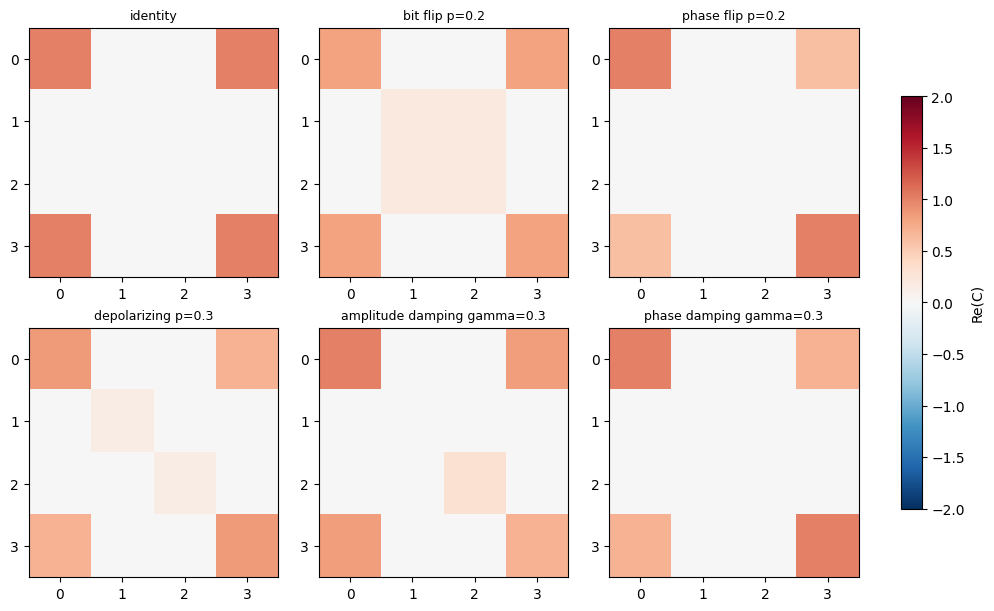
\includegraphics[width=0.94\textwidth]{fig_01_theory_01_cell6.png}
\caption{대표적인 qubit channel들의 Choi 행렬 실수부 비교. Identity channel은 계수가 1인 순수한 구조를 보이고, depolarizing channel은 대각 성분이 더 균일해지며, amplitude damping channel은 대칭적인 수축만이 아니라 특정 방향으로의 relaxation 구조가 나타난다. 이 그림은 채널의 물리적 성질이 Choi 행렬의 패턴에 직접 반영된다는 점을 보여준다.}
\label{fig:theory-choi-examples}
\end{figure}

그림 \ref{fig:theory-choi-examples}에서 가장 먼저 볼 것은 identity channel과 잡음 채널의 차이다. Identity channel(아무 일도 하지 않는 채널)의 Choi 행렬은 이상적인 최대 얽힘 구조를 가지므로, 특정 위치에 큰 결맞음(coherence) 성분이 또렷하게 남아 있다. 반면 depolarizing channel은 상태를 완전 무질서 상태 쪽으로 밀기 때문에 Choi 행렬의 뚜렷한 구조가 약해진다. 이것은 2.4절에서 본 ``Bloch 구가 모든 방향으로 균일하게 줄어드는'' 현상과 같은 내용이다.

Amplitude damping channel은 depolarizing과 달리 단순한 균일 수축으로 설명되지 않는다. 이 채널은 들뜬 상태가 바닥 상태로 내려가는 relaxation을 나타내므로 완전 무질서 상태조차 그대로 보존하지 않는다. 따라서 TP 조건은 만족하지만 unital 조건은 만족하지 않는다(2.5절의 개념 상자). 이 결과는 TP와 unitality가 서로 다른 조건임을 잘 보여준다: TP는 전체 확률이 보존된다는 뜻이고, unitality는 완전 무질서 상태가 보존된다는 뜻이다. 그림에서 보이는 이 차이가 실제 \emph{계산}에서도 같은 결론으로 이어지는지 확인하기 위해, 다음으로 CP/TP 판정과 표현 변환 오차를 수치로 비교했다.

\subsection{수치 검증 결과: 변환이 정말 일치하는가}

표 \ref{tab:theory-results}는 이론 파트에서 확인한 대표적인 수치 결과다. 결과를 읽기 전에 한 가지 숫자 감각을 짚어 두자.

\begin{conceptbox}{개념: ``오차 $10^{-16}$''이 무슨 뜻인가}
컴퓨터는 실수를 유한한 자릿수(double precision, 약 16자리 십진수)로만 저장한다. 그래서 아무리 수학적으로 정확한 계산도 마지막 자리에서 미세한 \emph{반올림 오차(round-off error)}가 남는다. 그 크기가 대략 $10^{-16}$ 수준이다. 따라서 두 계산 결과의 차이가 $10^{-16}$ 정도라면, 그것은 ``오차가 있다''가 아니라 \emph{컴퓨터가 표현할 수 있는 한 완벽히 일치한다}는 뜻이다. 반대로 차이가 예컨대 $0.27$이라면 그것은 진짜 차이다.
\end{conceptbox}

\begin{table}[H]
\centering
\small
\begin{tabularx}{\textwidth}{p{0.25\textwidth}p{0.31\textwidth}X}
\toprule
항목 & 관측값 & 해석 \\
\midrule
Identity channel & Choi rank $=1$ & 하나의 Kraus operator로 충분하므로 잡음 branch가 없다. \\
Depolarizing $p=0.3$ & min eigenvalue $=0.15$, TP=True, unital=True & 모든 Choi 고유값이 음수가 아니므로 CP이며, maximally mixed state를 보존한다. \\
Amplitude damping $\gamma=0.3$ & TP=True, unital=False, rank $=2$ & 확률은 보존하지만 Bloch sphere 중심이 이동하므로 unital하지 않다. \\
Random channel round-trip & error $\approx2.56\times10^{-16}$ & Choi에서 Kraus로 복원해도 원래 채널 작용과 machine precision 수준에서 일치한다. \\
Composition check & error $\approx2.48\times10^{-16}$ & natural form의 행렬곱이 channel composition과 일치한다. \\
\bottomrule
\end{tabularx}
\caption{이론 파트의 주요 수치 검증 결과}
\label{tab:theory-results}
\end{table}

표를 한 줄씩 읽어 보자. \emph{Identity channel}의 Choi 계수가 1이라는 것은 잡음 갈래가 없는 깨끗한 unitary라는 뜻이다(4.1절 개념 상자). \emph{Depolarizing}의 최소 고유값이 $0.15>0$이므로 모든 고유값이 음이 아니어서 CP이고, unital도 True다. \emph{Amplitude damping}은 TP=True지만 unital=False로 나와, 앞 절의 그림 해석(중심 이동)을 수치가 그대로 확인해 준다. 마지막 두 줄, \emph{round-trip}(Choi$\to$Kraus$\to$다시 작용)과 \emph{composition}(natural 표현 곱셈) 오차가 $10^{-16}$ 수준이라는 것은 위 개념 상자에 따라 ``네 가지 표현이 서로 완벽히 일치한다''는 결론이다.

특히 perturbed identity(아주 살짝 흔든 항등 채널)의 Choi 행렬이 CP=False로 판정된 예시는 중요하다. 행렬이 에르미트이고 대각합 조건을 거의 만족하더라도, 아주 작은 \emph{음의} 고유값 하나가 존재하면 완전양성성이 깨진다. 이는 tomography에서 raw reconstruction(가공하지 않은 재구성)을 그대로 믿으면 안 되는 이유와 직접 연결된다. 실제 실험에서는 측정 횟수가 유한해 생기는 \textbf{shot noise} 때문에 선형 역산 결과가 물리적으로 불가능한 Choi 행렬(음의 고유값을 가진)을 만들 수 있고, 이 경우에는 가장 가까운 물리적 채널로 되돌리는 \textbf{CPTP projection}이 필요하다. 이것이 바로 다음 장의 주제다.

%==================================================================
\section{작업 2 --- Process Tomography와 Choi 행렬 재구성}
%==================================================================

\subsection{먼저 알아야 할 것: tomography가 왜 필요한가}

이론적으로 정의한 채널의 Choi 행렬은 코드로 바로 계산할 수 있다. 그러나 실제 장치에서 \emph{어떤} 채널이 작용했는지는 직접 알 수 없다. 예를 들어 $X$ 게이트(큐비트를 뒤집는 NOT에 해당)를 실행했다 해도, 실제로는 이상적인 $X$ 뒤에 amplitude damping, depolarizing 잡음, coherent error가 섞여 있을 수 있다.

\begin{conceptbox}{개념: process tomography (과정 단층촬영)}
``단층촬영''은 여러 각도에서 찍은 정보를 합쳐 내부 구조를 복원하는 기법이다(의료 CT처럼). \textbf{process tomography}는 알 수 없는 채널에 \emph{여러 가지 입력 상태}를 넣고 \emph{출력 상태들을 측정}한 뒤, 그 데이터로부터 ``장치가 실제로 구현한 채널''의 Choi 행렬을 복원한다. 즉 채널이라는 블랙박스의 내부를 사진(Choi 행렬)으로 재구성하는 것이다.
\end{conceptbox}

이 작업에서는 IBM 하드웨어 실행을 염두에 둔 구조를 만들되, 보고서의 \emph{재현성}을 위해 실제 하드웨어 대신 \textbf{오프라인 모의 데이터(offline simulated data)}를 사용했다. 이 선택은 실제 하드웨어 성능을 주장하기 위한 것이 아니라, tomography 파이프라인이 물리적으로 일관되게 작동하는지를 검증하기 위한 것이다. 하드웨어 결과는 backend 보정 상태, 대기열(queue), 측정 횟수(shot count)에 따라 매번 달라지므로, 먼저 고정된 데이터(fixture)로 계산 흐름을 검증하는 것이 적절하다.

모의 실험에서 기준이 되는 게이트는 Qiskit \texttt{QuantumCircuit}으로 정의했다. 그림 \ref{fig:qpt-target-circuits}의 $X$, $H$, CNOT 회로는 이상적인(ideal) Choi 행렬을 만들 때 쓰는 \emph{기준 회로}다. 이후의 모의 잡음 채널은 이 이상적 회로 자체를 바꾸는 것이 아니라, 기준 게이트 \emph{뒤에} amplitude damping이나 depolarizing 채널을 붙인 ``대역(stand-in) 채널''로 구성했다. 따라서 회로도는 tomography가 어떤 게이트를 기준으로 비교하는지를 보여주고, 뒤의 Choi heatmap과 fidelity 표는 그 기준에 잡음이 섞이면 재구성 결과가 어떻게 달라지는지를 보여준다.

\begin{conceptbox}{개념: $X$, $H$, CNOT 게이트}
\textbf{$X$ 게이트}: $|0\rangle\leftrightarrow|1\rangle$을 뒤집는 양자 NOT. \textbf{$H$ 게이트(아다마르)}: $|0\rangle,|1\rangle$을 균등 중첩으로 만드는 게이트(중첩의 대표). \textbf{CNOT}: 제어 큐비트 $q_0$가 $|1\rangle$일 때만 대상 큐비트 $q_1$을 뒤집는 \emph{두 큐비트} 게이트로, 얽힘을 만드는 데 쓰인다. 앞의 둘은 1큐비트, CNOT은 2큐비트라는 점이 뒤의 결과 해석에서 중요하다.
\end{conceptbox}

\begin{figure}[H]
\centering
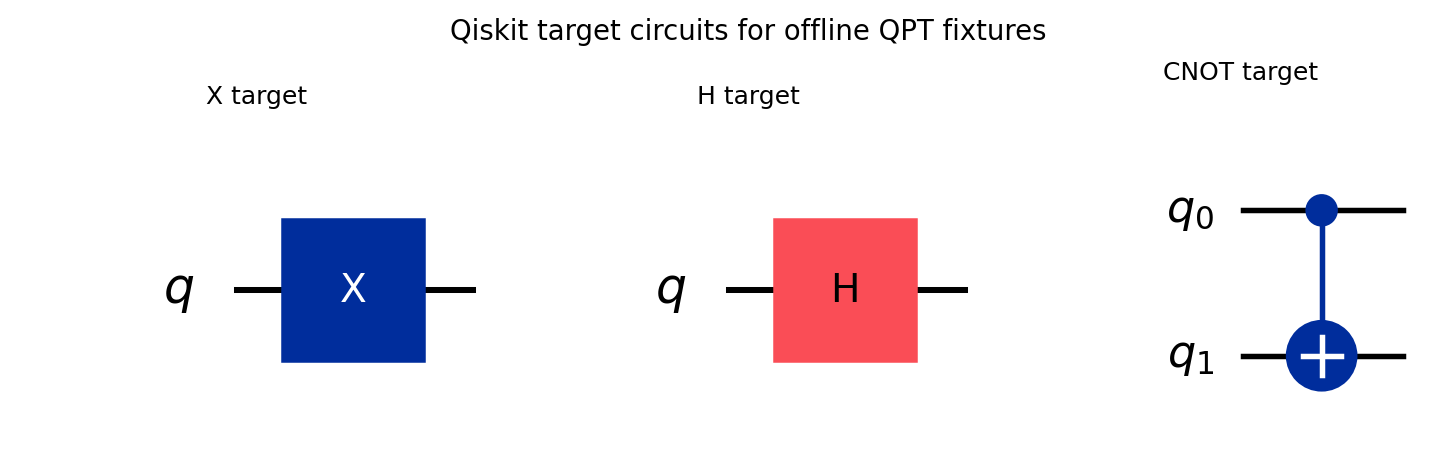
\includegraphics[width=0.92\textwidth]{fig_02_ibm_experiment_00_qiskit_circuits.png}
\caption{Offline QPT fixture에서 사용하는 Qiskit target circuits. $X$와 $H$는 one-qubit gate이고, CNOT은 control qubit $q_0$와 target qubit $q_1$에 작용하는 two-qubit gate이다. Noise model은 회로 안에 추가 gate로 그리지 않고, 이 target gate 뒤에 작용하는 Choi-level channel로 적용하였다.}
\label{fig:qpt-target-circuits}
\end{figure}

\subsection{이상적인 Choi 행렬 대 재구성된 Choi 행렬}

tomography 결과를 해석할 때 가장 먼저 확인할 것은, 재구성된 Choi 행렬이 이상적인 Choi 행렬의 \emph{큰 구조}를 유지하는가이다. 큰 구조가 완전히 사라졌다면 게이트가 원하는 작용과 전혀 다른 일을 한 것이고, 큰 구조는 유지되되 작은 성분이 달라졌다면 이상적인 작용 위에 잡음이 얹힌 것으로 읽을 수 있다. 이 구분을 위해 먼저 $X$ 게이트의 ideal Choi와 reconstructed Choi를 나란히 비교했다.

\begin{figure}[H]
\centering
\begin{subfigure}{0.48\textwidth}
\centering
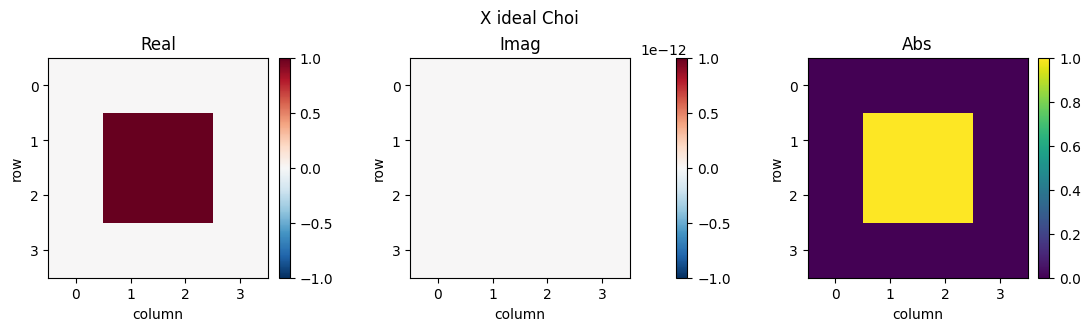
\includegraphics[width=\textwidth]{fig_02_ibm_experiment_01_cell20.png}
\caption{$X$ ideal Choi}
\end{subfigure}
\hfill
\begin{subfigure}{0.48\textwidth}
\centering
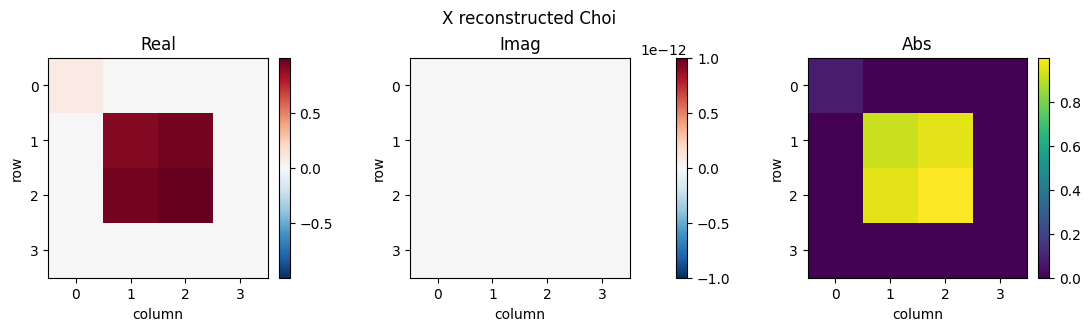
\includegraphics[width=\textwidth]{fig_02_ibm_experiment_02_cell20.png}
\caption{$X$ reconstructed Choi}
\end{subfigure}
\caption{$X$ gate의 이상적인 Choi 행렬과 재구성된 Choi 행렬 비교. 두 그림의 큰 구조는 비슷하지만 재구성된 행렬에서는 ideal pattern에서 벗어난 작은 성분들이 나타난다. 이는 gate가 완전히 틀렸다는 뜻이 아니라, 이상적인 unitary 과정에 잡음 성분이 섞였다는 뜻으로 해석된다.}
\label{fig:qpt-x-choi}
\end{figure}

그림 \ref{fig:qpt-x-choi}에서 reconstructed Choi가 ideal Choi와 완전히 같지 않은 것은 자연스럽다. 만약 두 행렬이 완전히 같다면 process fidelity는 1에 가깝고 diamond distance는 0에 가까워야 한다. 이 두 지표를 먼저 정의하자.

\begin{conceptbox}{개념: 두 가지 비교 지표 --- fidelity와 diamond distance}
\textbf{Process fidelity $F_{\mathrm{pro}}$}와 \textbf{average gate fidelity $F_{\mathrm{avg}}$}는 ``두 채널이 \emph{평균적으로} 얼마나 비슷한가''를 0과 1 사이 숫자로 요약한다. 1에 가까울수록 비슷하다. 평균적 유사도이므로, 운 나쁜 특정 입력에서 얼마나 차이 나는지는 가려진다.

\textbf{Diamond distance}(정확히는 half-diamond distance)는 ``\emph{최악의 경우}, 즉 두 채널을 가장 잘 구별하는 입력을 골랐을 때 얼마나 다른가''를 잰다. 0이면 어떤 입력으로도 구별 불가, 클수록 구별 쉬움. 6장에서 이 양이 채널 구별 성공확률과 직접 연결된다.
\end{conceptbox}

실제 결과에서 $X$ 게이트의 process fidelity는 $0.959583$으로 비교적 높았지만, half-diamond distance는 $0.080000$으로 0이 아니었다. 따라서 \emph{평균적으로는} 이상적 $X$와 상당히 가깝지만, \emph{최적의 입력 상태를 고르면} 구별 가능한 차이가 남아 있다는 뜻이다. 두 지표가 ``비슷하다''와 ``그래도 차이가 있다''를 각각 다른 각도에서 말해 주는 셈이다.

$X$ 게이트 하나만 보면 이 차이가 특정 게이트만의 일인지, 전체에서 반복되는 경향인지 알기 어렵다. 그래서 다음으로 $X$, $H$, CNOT 세 게이트를 같은 지표로 비교했다. 이는 1큐비트 게이트와 2큐비트 게이트에서 잡음 크기가 어떻게 다르게 나타나는지 보기 위한 것이다.

\begin{figure}[H]
\centering
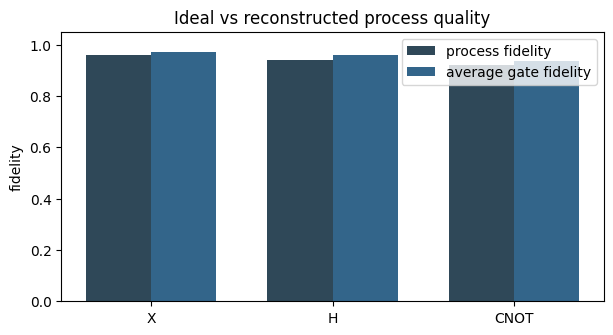
\includegraphics[width=0.74\textwidth]{fig_02_ibm_experiment_10_cell24.png}
\caption{$X$, $H$, CNOT에 대한 process fidelity와 average gate fidelity 비교. 모든 경우에서 fidelity가 1보다 작으므로 noise가 존재하며, CNOT의 fidelity가 상대적으로 낮게 나온다. 이는 two-qubit channel이 one-qubit channel보다 차원이 크고 noise branch가 많아지기 때문으로 생각된다.}
\label{fig:qpt-fidelity-bars}
\end{figure}

그림 \ref{fig:qpt-fidelity-bars}에서 CNOT의 process fidelity가 가장 낮았다. 이는 CNOT이 두 큐비트에 작용하므로 Choi 행렬의 차원이 커지고(2큐비트라 $16\times16$), 전역 depolarizing 잡음이 붙으면 가능한 Pauli error 갈래의 수가 많아지기 때문이다. 따라서 똑같은 잡음 세기처럼 보여도 2큐비트 게이트에서는 오차가 더 많은 방향으로 퍼질 수 있다. 이 결과를 실제 하드웨어 성능이라고 결론 내릴 수는 없지만, 분석 파이프라인이 1큐비트와 2큐비트 과정을 같은 방식으로 비교할 수 있음을 보여준다.

\subsection{잡음의 ``방향''까지 보기: Bloch 구 변형}

다만 fidelity 막대그래프만으로는 잡음이 \emph{어떤 방향}으로 작용했는지 알 수 없다. fidelity가 비슷하게 낮아져도, 한 경우는 모든 방향으로 균일하게 수축했을 수 있고 다른 경우는 특정 축으로 상태가 이동했을 수 있다. 이 차이를 보기 위해 1큐비트 채널에 대해서는 Bloch 구 변형(2.4절)을 함께 보았다.

\begin{figure}[H]
\centering
\begin{subfigure}{0.47\textwidth}
\centering
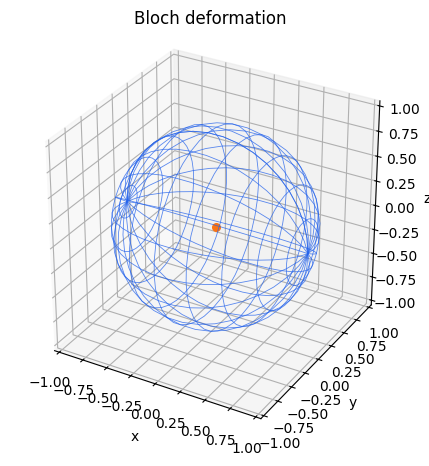
\includegraphics[width=0.82\textwidth]{fig_02_ibm_experiment_07_cell22.png}
\caption{$X$ reconstructed channel}
\end{subfigure}
\hfill
\begin{subfigure}{0.47\textwidth}
\centering
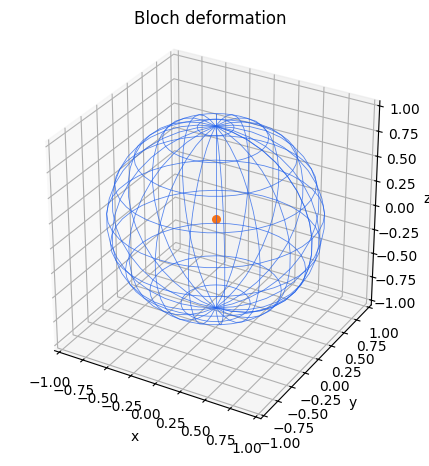
\includegraphics[width=0.82\textwidth]{fig_02_ibm_experiment_08_cell22.png}
\caption{$H$ reconstructed channel}
\end{subfigure}
\caption{재구성된 one-qubit channel의 Bloch sphere 변형. Depolarizing-like noise는 전체 구를 비교적 균일하게 줄이는 반면, amplitude-damping-like relaxation은 중심 이동을 동반한다. 따라서 Bloch sphere 그림은 fidelity 숫자만으로 보이지 않는 noise의 방향성을 보여준다.}
\label{fig:qpt-bloch}
\end{figure}

그림 \ref{fig:qpt-bloch}는 fidelity만으로는 설명하기 어려운 부분을 보완한다. fidelity는 하나의 숫자로 평균적 유사도를 말해 주지만, 잡음이 어느 방향으로 작용하는지는 보여주지 않는다. 반면 Bloch 구 변형을 보면 구가 균일하게 줄어드는지, 특정 방향으로 이동하는지, 특정 축이 더 많이 줄어드는지 알 수 있다. $X$ 게이트에서 amplitude-damping-like relaxation이 진단된 것은 중심 이동과 관련이 있고, $H$ 게이트에서 depolarizing-like 수축이 나타난 것은 방향성 있는 이동보다 전체적 수축이 두드러졌기 때문이다.

이 진단은 그림만 보고 정성적으로 붙인 이름표가 아니라, 재구성된 Choi 행렬을 Pauli-transfer 표현으로 바꾼 뒤 Bloch 아핀 작용을 계산하여 얻은 것이다. 이상적 게이트의 작용을 제거한 \emph{잔차(residual) 채널}을 2.4절의 아핀 형태
\[
\vec r\mapsto M\vec r+\vec t
\]
로 보았을 때, 중심 이동 $\vec t$의 크기가 크면 relaxation-like 잡음으로, $\vec t$가 거의 0이면서 $M$의 특이값(singular value)들이 거의 같은 비율로 작아지면 depolarizing-like 수축으로 분류했다. 표 \ref{tab:qpt-bloch-diagnostics}는 이 기준에 쓰인 수치값이다.

\begin{table}[H]
\centering
\small
\begin{tabularx}{\textwidth}{lcccX}
\toprule
Gate & $\|t\|_2$ & Singular-value spread & Mean shrinkage & 진단 근거 \\
\midrule
$X$ & 0.07999965 & 0.03916625 & 0.94611071 & 중심 이동 norm이 threshold 0.05보다 크므로 amplitude-damping-like relaxation으로 분류된다. \\
$H$ & $1.999\times10^{-15}$ & $1.999\times10^{-12}$ & 0.92000000 & 중심 이동과 축별 spread가 거의 0이고 전체 수축이 뚜렷하므로 depolarizing-like isotropic shrinkage로 분류된다. \\
\bottomrule
\end{tabularx}
\caption{One-qubit reconstructed channel의 Bloch affine 진단 수치. $\|t\|_2$는 Bloch sphere 중심 이동의 크기이고, singular-value spread는 세 Bloch 축의 수축 정도가 서로 얼마나 다른지를 나타낸다.}
\label{tab:qpt-bloch-diagnostics}
\end{table}

표 \ref{tab:qpt-bloch-diagnostics}를 읽어 보자. $X$는 중심 이동 $\|t\|_2\approx0.08$로 기준값 $0.05$보다 크므로 ``중심이 옮겨갔다'' $\to$ relaxation으로 분류된다. $H$는 $\|t\|_2$가 $10^{-15}$로 사실상 0이고 축별 차이(spread)도 $10^{-12}$로 0이며 전체 수축만 뚜렷하므로 ``중심 고정, 균일 수축'' $\to$ depolarizing으로 분류된다. 4.3절의 개념 상자를 떠올리면 $10^{-15}$는 ``0과 같다''는 뜻임을 알 수 있다.

따라서 tomography 결과는 \emph{세 가지를 함께} 보아야 안정적으로 해석된다: Choi heatmap은 이상적 과정과 재구성 과정의 \emph{구조적} 차이를, fidelity는 그 차이를 \emph{한 숫자}로, Bloch 구는 그 차이가 어떤 \emph{물리적 잡음 모양}인지를 보여준다. 세 관찰을 종합한 값이 표 \ref{tab:qpt-results}이다.

\begin{table}[H]
\centering
\small
\begin{tabularx}{\textwidth}{lcccX}
\toprule
Gate & $F_{\mathrm{pro}}$ & $F_{\mathrm{avg}}$ & Half-diamond distance & 진단 \\
\midrule
$X$ & 0.959583 & 0.973055 & 0.080000 & amplitude-damping-like relaxation \\
$H$ & 0.940000 & 0.960000 & 0.060000 & depolarizing-like isotropic shrinkage \\
CNOT & 0.920000 & 0.936000 & 0.080000 & stochastic global depolarizing-like noise \\
\bottomrule
\end{tabularx}
\caption{Offline simulated QPT 결과}
\label{tab:qpt-results}
\end{table}

마지막으로, 4.3절 끝에서 예고한 ``물리적으로 불가능한 재구성'' 문제를 확인하자. Linear inversion(선형 역산) perturbation 예시에서는 최소 고유값이 $-0.270000$으로 나와 CP 조건이 깨졌다. 이 값은 단순한 수치 오차라기에는 너무 크다($10^{-16}$이 아니라 $0.27$이다 --- 4.3절 개념 상자). 따라서 raw reconstruction은 물리적 채널로 받아들일 수 없고, MLE(최대우도추정)나 CPTP projection으로 \emph{가장 가까운 물리적 Choi 행렬}을 찾아야 한다. 이 과정은 결과를 예쁘게 만들기 위한 후처리가 아니라, 밀도행렬과 채널이 반드시 만족해야 하는 물리 법칙(고유값이 음이 아님)을 회복하는 과정이다.

%==================================================================
\section{작업 3 --- Channel Discrimination과 SDP}
%==================================================================

\subsection{먼저 알아야 할 것: ``구별''은 ``비슷함''과 다른 문제다}

fidelity는 두 채널이 \emph{평균적으로} 얼마나 비슷한지 알려준다. 그러나 ``두 채널을 실제 실험에서 얼마나 잘 \emph{구별}할 수 있는가''는 별개의 문제다. 다음 상황을 생각하자: 동전을 던져 두 채널 $\E_0$, $\E_1$ 중 하나를 골라(각각 확률 $1/2$) 당신에게 준다. 당신은 그 채널에 원하는 입력을 넣고 출력을 측정해 ``어느 쪽이었나''를 맞혀야 한다. 이때 최선의 전략으로 맞힐 확률은 다음과 같다.

\begin{conceptbox}{개념: diamond norm과 구별 성공확률}
동일한 사전확률($1/2$씩)로 주어진 두 채널을 구별하는 최적 성공확률은
\[
p_{\mathrm{succ}}^{\max}=\frac12+\frac14\,\|\E_0-\E_1\|_\diamond .
\]
여기서 $\|\cdot\|_\diamond$가 \textbf{diamond norm}이다. 두 채널이 같으면 norm이 0이라 성공확률은 $1/2$(찍기와 동일), 두 채널이 ``완벽히 구별 가능''하면 norm이 2라 성공확률은 1이 된다. 결정적으로, diamond norm은 \emph{보이지 않는 참조계와의 얽힘까지 허용한} 최적 구별 능력을 잰다.
\end{conceptbox}

이 ``얽힘 허용''이 왜 중요한가? 입력을 \emph{단독(product)}으로만 줄 때와, 참조계와 \emph{얽힌(entangled)} 입력을 줄 때 성능이 달라질 수 있기 때문이다. 그리고 diamond norm은 SDP라는 최적화로 계산된다.

\begin{conceptbox}{개념: SDP (semidefinite programming, 반정부호 계획법)}
SDP는 ``어떤 행렬이 양의 준정부호($\succeq0$)여야 한다''는 제약 아래에서 어떤 양을 최대/최소화하는 최적화 문제다. 양자정보에서 ``물리적으로 가능한 채널/측정/상태''라는 제약이 바로 $\succeq0$ 형태이므로, 많은 최적 전략 문제가 SDP로 자연스럽게 표현된다. 핵심은 \textbf{Choi 행렬이 곧 SDP의 입력}이 된다는 점이다 --- 즉 Choi 표현이 단순한 기록 형식을 넘어 ``실험적으로 의미 있는 성공확률''과 직접 연결된다.
\end{conceptbox}

\subsection{가장 단순한 경우: 채널 차이가 커질수록 구별이 쉬워진다}

먼저 가장 해석하기 쉬운 경우로, depolarizing channel의 매개변수가 바뀔 때 성공확률이 어떻게 변하는지 보았다. 이 예시는 ``두 채널의 차이가 커질수록 구별이 쉬워진다''는 기본 직관을 확인하는 역할을 한다. 이 기본 경향이 확인되어야, 뒤에서 얽힘이나 반복 사용이 주는 추가 이점을 더 분명히 해석할 수 있다.

\begin{figure}[H]
\centering
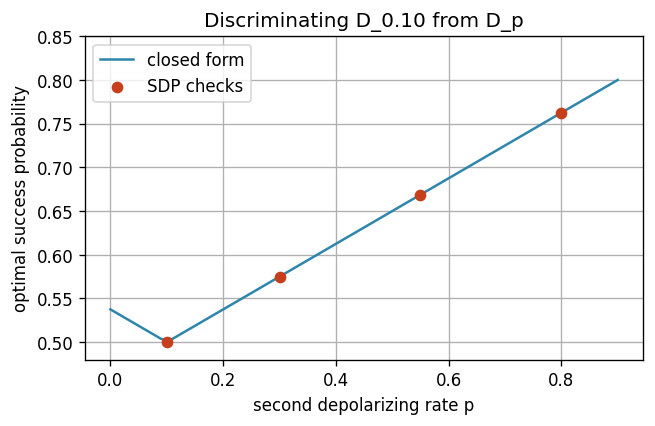
\includegraphics[width=0.72\textwidth]{fig_03_sdp_discrimination_01_cell9.png}
\caption{Depolarizing channel parameter가 달라질 때의 discrimination success probability. 기준 parameter와 비교 대상 parameter가 가까울수록 성공확률은 0.5에 가까워지고, 멀어질수록 성공확률이 증가한다. 이는 두 채널의 작용이 비슷하면 어떤 측정을 하더라도 구별하기 어렵다는 직관과 일치한다.}
\label{fig:sdp-depolarizing}
\end{figure}

그림 \ref{fig:sdp-depolarizing}에서 성공확률이 $0.5$ 근처라는 것은 ``찍기''와 큰 차이가 없다는 뜻이다. 기준 채널과 비교 채널의 depolarizing 세기가 거의 같으면 출력 상태의 차이가 작아져 구별이 어렵다. 반대로 매개변수 차이가 커질수록 출력 상태들이 더 많이 달라지고, 최적 측정의 성공확률도 증가한다.

\subsection{얽힘과 반복 사용의 이점}

이제 문제는 ``매개변수 차이가 크면 성공확률이 올라간다''에서 끝나지 않는다. \emph{같은} 두 채널을 구별하더라도 어떤 입력 전략을 쓰는지에 따라 성능이 달라진다. 특히 diamond norm은 참조계와의 얽힘까지 허용하므로, 단독 입력만 쓰는 경우와 \textbf{ancilla(보조 큐비트)-assisted} 입력을 쓰는 경우를 비교해야 한다.

\begin{figure}[H]
\centering
\begin{subfigure}{0.48\textwidth}
\centering
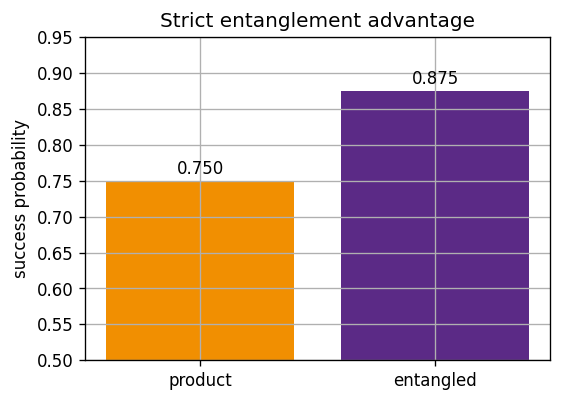
\includegraphics[width=\textwidth]{fig_03_sdp_discrimination_04_cell18.png}
\caption{Product input과 entangled input 비교}
\end{subfigure}
\hfill
\begin{subfigure}{0.48\textwidth}
\centering
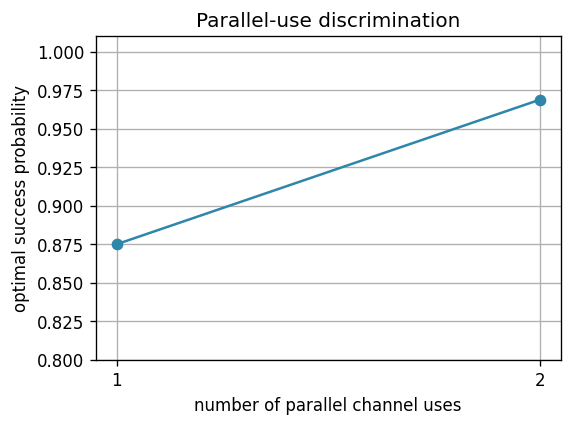
\includegraphics[width=\textwidth]{fig_03_sdp_discrimination_05_cell21.png}
\caption{Parallel channel use에 따른 성공확률}
\end{subfigure}
\caption{Channel discrimination에서 entanglement와 반복 사용이 주는 이점. Product input의 성공확률은 0.750000이었지만, ancilla-assisted input에서는 0.875000으로 증가하였다. 또한 2-shot parallel strategy에서는 0.968750까지 증가하였다.}
\label{fig:sdp-advantage}
\end{figure}

그림 \ref{fig:sdp-advantage}에서 단독 입력과 얽힌 입력의 차이는 단순한 계산상의 차이가 아니라 \textbf{operational advantage}(실제로 이득이 되는 차이)다. 단독 입력만 쓰면 채널이 계 자체에 남긴 차이만 볼 수 있다. 하지만 참조계와 얽힘을 만든 뒤 채널이 계 쪽에만 작용하게 하면, 채널의 작용이 \emph{합동 상태의 상관(correlation)}에도 흔적을 남긴다(2.2절의 얽힘). 이 추가 정보 덕분에 성공확률이 오른다 --- 0.750000에서 0.875000으로.

2-shot 결과가 0.968750까지 오른 것도 자연스럽다. 같은 채널을 \emph{여러 번} 쓸 수 있으면 한 번의 출력보다 더 많은 정보를 얻고, 두 채널의 차이가 누적된다. 다만 이 방법은 채널 사용 횟수가 늘수록 Hilbert 공간 차원이 빠르게 커진다. 따라서 작은 예제에서는 효과가 명확하지만, 큰 계에서는 SDP의 계산 비용이 곧 한계가 된다. 이 관찰들을 수치로 정리하면 표 \ref{tab:sdp-results}와 같다. 표는 Choi 행렬을 사용한 SDP가 단순한 유사도 계산이 아니라 \emph{실제 구별 전략의 성공확률}을 비교하는 도구임을 보여준다.

\begin{table}[H]
\centering
\begin{tabular}{lcc}
\toprule
전략 & 성공확률 & 해석 \\
\midrule
Bit-flip closed-form 검증 & 0.625000 & analytical diamond norm과 SDP 결과가 일치한다. \\
Product input & 0.750000 & reference 없이 가능한 최선의 성능이다. \\
Ancilla-assisted input & 0.875000 & entanglement가 구별 능력을 높인다. \\
2-shot parallel & 0.968750 & channel use가 늘어나며 차이가 누적된다. \\
\bottomrule
\end{tabular}
\caption{SDP 기반 channel discrimination의 주요 결과}
\label{tab:sdp-results}
\end{table}

표 \ref{tab:sdp-results}의 첫 줄(bit-flip closed-form 검증)은 손으로 풀 수 있는 간단한 경우의 \emph{해석적} diamond norm 값과 SDP 수치가 일치함을 확인한 것이다 --- 즉 SDP 구현 자체가 옳다는 신뢰성 점검이다. 나머지 세 줄은 전략을 강화할수록($0.75\to0.875\to0.969$) 성공확률이 단조 증가함을 보여준다.

%==================================================================
\section{작업 4 --- Non-Markovian Dynamics와 Quantum Combs}
%==================================================================

\subsection{먼저 알아야 할 것: 단일 시점 채널의 한계}

지금까지의 Choi 행렬은 \emph{하나의} 입력-출력 관계를 설명했다. 그러나 시간에 따라 진행되는 과정에서, 계가 환경과 여러 번 상호작용하고 그 환경이 다음 시점에도 \emph{기억}을 갖고 남아 있다면, 단일 시점 채널만으로 전체 과정을 설명하기 어렵다.

\begin{conceptbox}{개념: Markovian 대 non-Markovian (기억 효과)}
\textbf{Markovian} 과정은 ``기억이 없는'' 과정이다 --- 미래는 오직 현재 상태에만 의존하고, 과거의 흔적은 남지 않는다. 잡음이 환경으로 \emph{한 번 새어 나가면 다시 돌아오지 않는} 경우다. \textbf{non-Markovian} 과정은 ``기억이 있는'' 과정으로, 환경에 저장된 정보가 나중에 계로 \emph{되돌아올} 수 있다. 각 시점의 부분 채널(marginal channel)은 모두 정상적인 CPTP 채널처럼 보여도, 시점들 사이에 시간 상관이 남아 있으면 전체 과정은 ``기억 없는 곱(memoryless product)''으로 분해되지 않는다.
\end{conceptbox}

\begin{conceptbox}{개념: quantum comb (양자 빗)}
이런 다중 시점 과정을 다루려면 \textbf{quantum comb} 또는 process tensor 관점이 필요하다. quantum comb는 여러 time slot의 입력-출력 관계를 하나의 큰 ``Choi 같은(Choi-like)'' 연산자로 묶는다. 이름이 ``빗''인 것은 시간 축을 따라 입력/출력 단자(이빨)가 늘어선 모양이기 때문이다. 단일 채널에서는 보이지 않던 시간 상관, 기억 잔여물(memory residue), 분해 실패(factorization failure)를 여기서 확인할 수 있다.
\end{conceptbox}

\subsection{기억 효과의 첫 신호: trace distance의 부활}

먼저 기억 효과가 실제 시간 신호에서 어떻게 보이는지 확인하기 위해 \textbf{trace distance}의 시간 변화를 보았다.

\begin{conceptbox}{개념: trace distance와 BLP witness}
\textbf{trace distance}는 두 상태를 ``얼마나 잘 구별할 수 있는가''를 재는 거리다(0이면 구별 불가, 클수록 구별 쉬움). 잡음 과정에서는 보통 시간이 지날수록 두 상태가 비슷해져 trace distance가 \emph{단조 감소}한다. 만약 중간에 \emph{다시 증가}한다면, 한때 환경으로 빠져나갔던 구별 정보가 계로 되돌아온 것 --- 즉 기억 효과의 증거다. \textbf{BLP witness}(Breuer--Laine--Piilo)는 바로 이 ``증가 구간''을 합산해 non-Markovian 정도를 수치화한 양이다.
\end{conceptbox}

\begin{figure}[H]
\centering
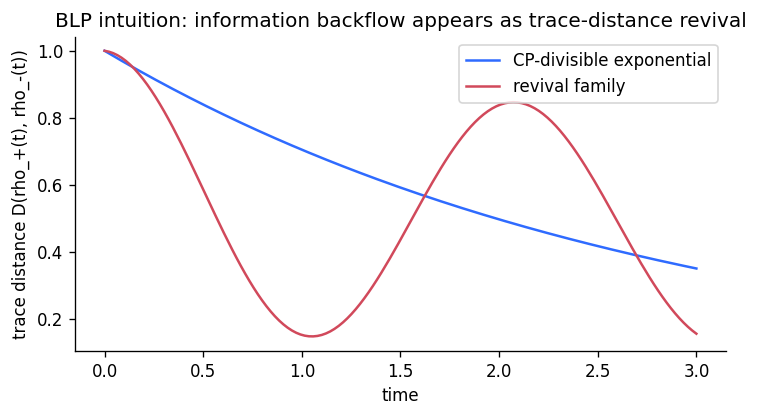
\includegraphics[width=0.76\textwidth]{fig_04_quantum_combs_01_cell7.png}
\caption{Markovian dephasing과 revival dephasing에서 trace distance의 시간 변화. Markovian dephasing에서는 trace distance가 단조 감소하지만, revival dephasing에서는 중간에 다시 증가하는 구간이 나타난다. 이 증가는 environment로 빠져나갔던 정보가 system으로 되돌아오는 현상으로 해석된다.}
\label{fig:comb-trace-distance}
\end{figure}

그림 \ref{fig:comb-trace-distance}에서 exponential dephasing의 trace distance는 계속 줄어든다 --- 두 상태를 구별할 정보가 시간이 지나며 사라지는 Markovian 상황이다. 반대로 revival dephasing에서는 trace distance가 \emph{다시 증가}하는 구간이 있다. 이 증가는 단순한 잡음 증가가 아니라, 이전에 환경으로 흘러나갔던 정보가 계로 일부 되돌아온 것이고, 따라서 BLP witness가 양의 값을 갖는다.

\subsection{구조적 증거: comb와 memoryless product의 차이}

그러나 trace distance 곡선만으로는 다중 시점 과정 \emph{전체}의 구조를 볼 수 없다. 정보가 되돌아오는 현상을 더 구조적으로 확인하려면, 각 time slot을 따로 보는 대신 전체 ``두 번 사용(two-use)'' 과정을 하나의 comb로 놓고 기억 없는 곱과 비교해야 한다.

\begin{figure}[H]
\centering
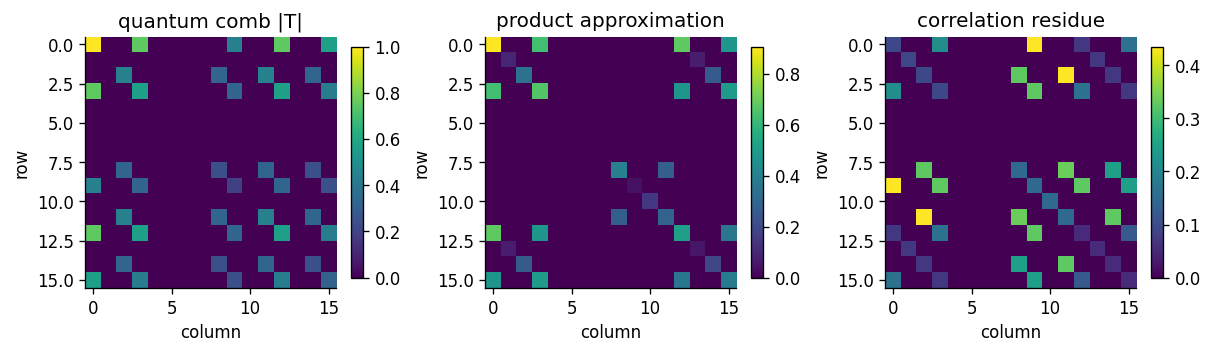
\includegraphics[width=0.92\textwidth]{fig_04_quantum_combs_02_cell10.png}
\caption{Two-use collision model에서 얻은 comb, memoryless product comb, 그리고 두 행렬의 차이. 두 marginal channel이 각각 물리적이더라도 전체 comb가 product form과 다르면 time slot 사이의 correlation이 남아 있다는 뜻이다.}
\label{fig:comb-correlation}
\end{figure}

\begin{conceptbox}{개념: collision model (충돌 모형)}
\textbf{collision model}은 기억 효과를 만드는 간단한 장난감 모형이다. 계가 환경 입자들과 차례로 ``충돌''(상호작용)하는데, \emph{같은 환경을 재사용}하면 첫 충돌의 흔적이 환경에 남아 다음 충돌에 영향을 준다. 이렇게 ``환경 재사용''이 기억의 원천이 된다.
\end{conceptbox}

그림 \ref{fig:comb-correlation}은 quantum comb 분석의 핵심을 보여준다. 왼쪽은 실제 collision model에서 얻은 \emph{전체} 과정(comb), 가운데는 각 time slot의 부분 채널을 단순히 곱해 만든 \emph{기억 없는} 근사(memoryless product), 오른쪽은 둘의 차이다. 오른쪽 차이가 0이 아니라는 것은, 전체 과정이 ``독립적인 두 채널의 연속''으로 설명되지 않는다 --- 즉 기억이 있다는 뜻이다.

수치로 보면 comb 행렬의 크기는 $16\times16$이었고, 최소 고유값은 $-1.774\times10^{-16}$이었다. 이 값은 음수지만 4.3절의 의미에서 \emph{사실상 0}(double precision 반올림 한계)이므로 물리적으로 0으로 보는 것이 타당하다 --- 즉 구성된 comb는 정당한(CP) 연산자다. 또한 결정적(deterministic) comb의 인과성 위계(causality hierarchy)도 True로 확인되었다. 반면 product marginal factorization은 False였고, 상대적 comb 상관 norm(relative comb correlation norm)은 약 $0.5307$이었다. \textbf{이 값이 0이 아니라는 점이 기억 효과의 핵심 증거다.}

여기서 주의할 점은, 각 time slot의 부분 채널이 \emph{이상해 보여서} 기억 효과가 생기는 것이 아니라는 것이다. 오히려 부분 채널은 각각 멀쩡한 1단계 채널처럼 보일 수 있다. 그래서 다음 그림에서는 부분 Choi 행렬만 따로 볼 때와 전체 comb를 볼 때의 차이를 확인했다.

\begin{figure}[H]
\centering
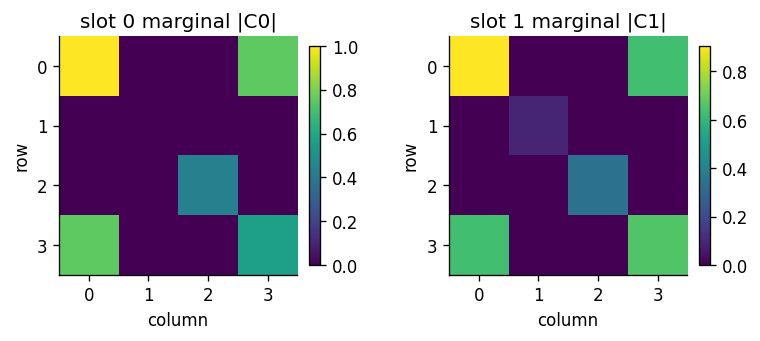
\includegraphics[width=0.72\textwidth]{fig_04_quantum_combs_03_cell13.png}
\caption{Two-use comb의 각 slot marginal Choi 행렬. 각 marginal만 보면 정상적인 single-step channel처럼 보이지만, marginal들의 곱만으로 전체 comb를 재구성할 수 없었다. 따라서 memory effect는 개별 시점의 채널이 아니라 시점 사이의 correlation에서 나타난다.}
\label{fig:comb-marginals}
\end{figure}

그림 \ref{fig:comb-marginals}는 왜 부분 채널만 보는 것이 부족한지 보여준다. 각 slot의 Choi 행렬은 그 자체로는 별 문제가 없어 보인다. 그러나 전체 comb와 product comb를 비교하면 차이가 남는다. 이는 실험에서 \emph{매 시점마다 멀쩡한 채널을 얻었다고 해서 전체 과정이 Markovian이라고 결론 내릴 수 없다}는 뜻이다. 이 결론은 앞의 trace distance 부활과 같은 방향을 가리킨다. 따라서 마지막으로 BLP와 RHP-style witness 값을 함께 정리해, 곡선 기반 진단과 comb 기반 진단이 서로 모순되지 않는지 확인했다.

\begin{conceptbox}{개념: RHP-style witness (CP-divisibility)}
\textbf{RHP witness}(Rivas--Huelga--Plenio)는 BLP와는 다른 각도에서 기억을 잡아낸다. ``전체 과정을 중간 시점들로 쪼갰을 때, \emph{각 중간 단계}가 그 자체로 정당한 CP 채널인가''를 본다. 정당하면 그 과정은 ``CP-divisible''(Markovian의 한 정의)이고, 중간 단계 중 하나라도 CP를 위반하면 non-Markovian이다. BLP가 ``정보가 되돌아오는가''를 본다면, RHP는 ``중간 단계가 물리적으로 쪼개지는가''를 본다.
\end{conceptbox}

\begin{table}[H]
\centering
\begin{tabular}{lcc}
\toprule
Channel family & BLP grid estimate & RHP-style grid witness \\
\midrule
Exponential dephasing & 0.000000 & 0.000000 \\
Revival dephasing & 0.699240 & 0.896321 \\
\bottomrule
\end{tabular}
\caption{비마르코프성 witness 결과}
\label{tab:nonmarkov-results}
\end{table}

표 \ref{tab:nonmarkov-results}에서 exponential dephasing은 BLP와 RHP-style witness가 모두 0이다 --- trace distance가 다시 증가하지 않았고, 중간 단계에서도 CP-divisibility 위반이 없었다는 뜻이다. 반면 revival dephasing은 두 witness가 모두 양의 값을 가졌다. 즉 \emph{서로 독립적인 두 진단 방식이 같은 결론}(기억 있음)을 내놓았다 --- 이것이 결과를 신뢰할 수 있게 해 준다.

%==================================================================
\section{작업 5 --- Interactive Widget과 시각적 해석}
%==================================================================

Interactive widget은 Choi 행렬의 조건들을 \emph{시각적으로} 확인하기 위해 만들어졌다. 수식으로는 $C_{\E}\succeq0$와 $\Tr_B(C_{\E})=I_A$가 간단해 보이지만, 실제 채널 작용에서 이 조건들이 어떤 모양으로 나타나는지 곧바로 떠올리기는 쉽지 않다. Widget은 매개변수를 움직일 때 Choi heatmap, 고유값 스펙트럼(eigenspectrum), Kraus 표시, Bloch 구 변형, CP/TP 표시기가 \emph{동시에} 변하도록 구성되었다.

앞의 네 작업에서는 Choi 행렬을 이론 검증, tomography, SDP, comb 분석에 각각 따로 사용했다. Widget은 이 계산들을 흩어진 결과로 두지 않고 \emph{한 화면에서 연결}한다는 점에서 의미가 있다. 예를 들어 amplitude damping을 선택하면 Choi 행렬의 패턴과 고유값뿐 아니라 Bloch 구가 어느 방향으로 변형되는지도 동시에 볼 수 있다.

\begin{figure}[H]
\centering
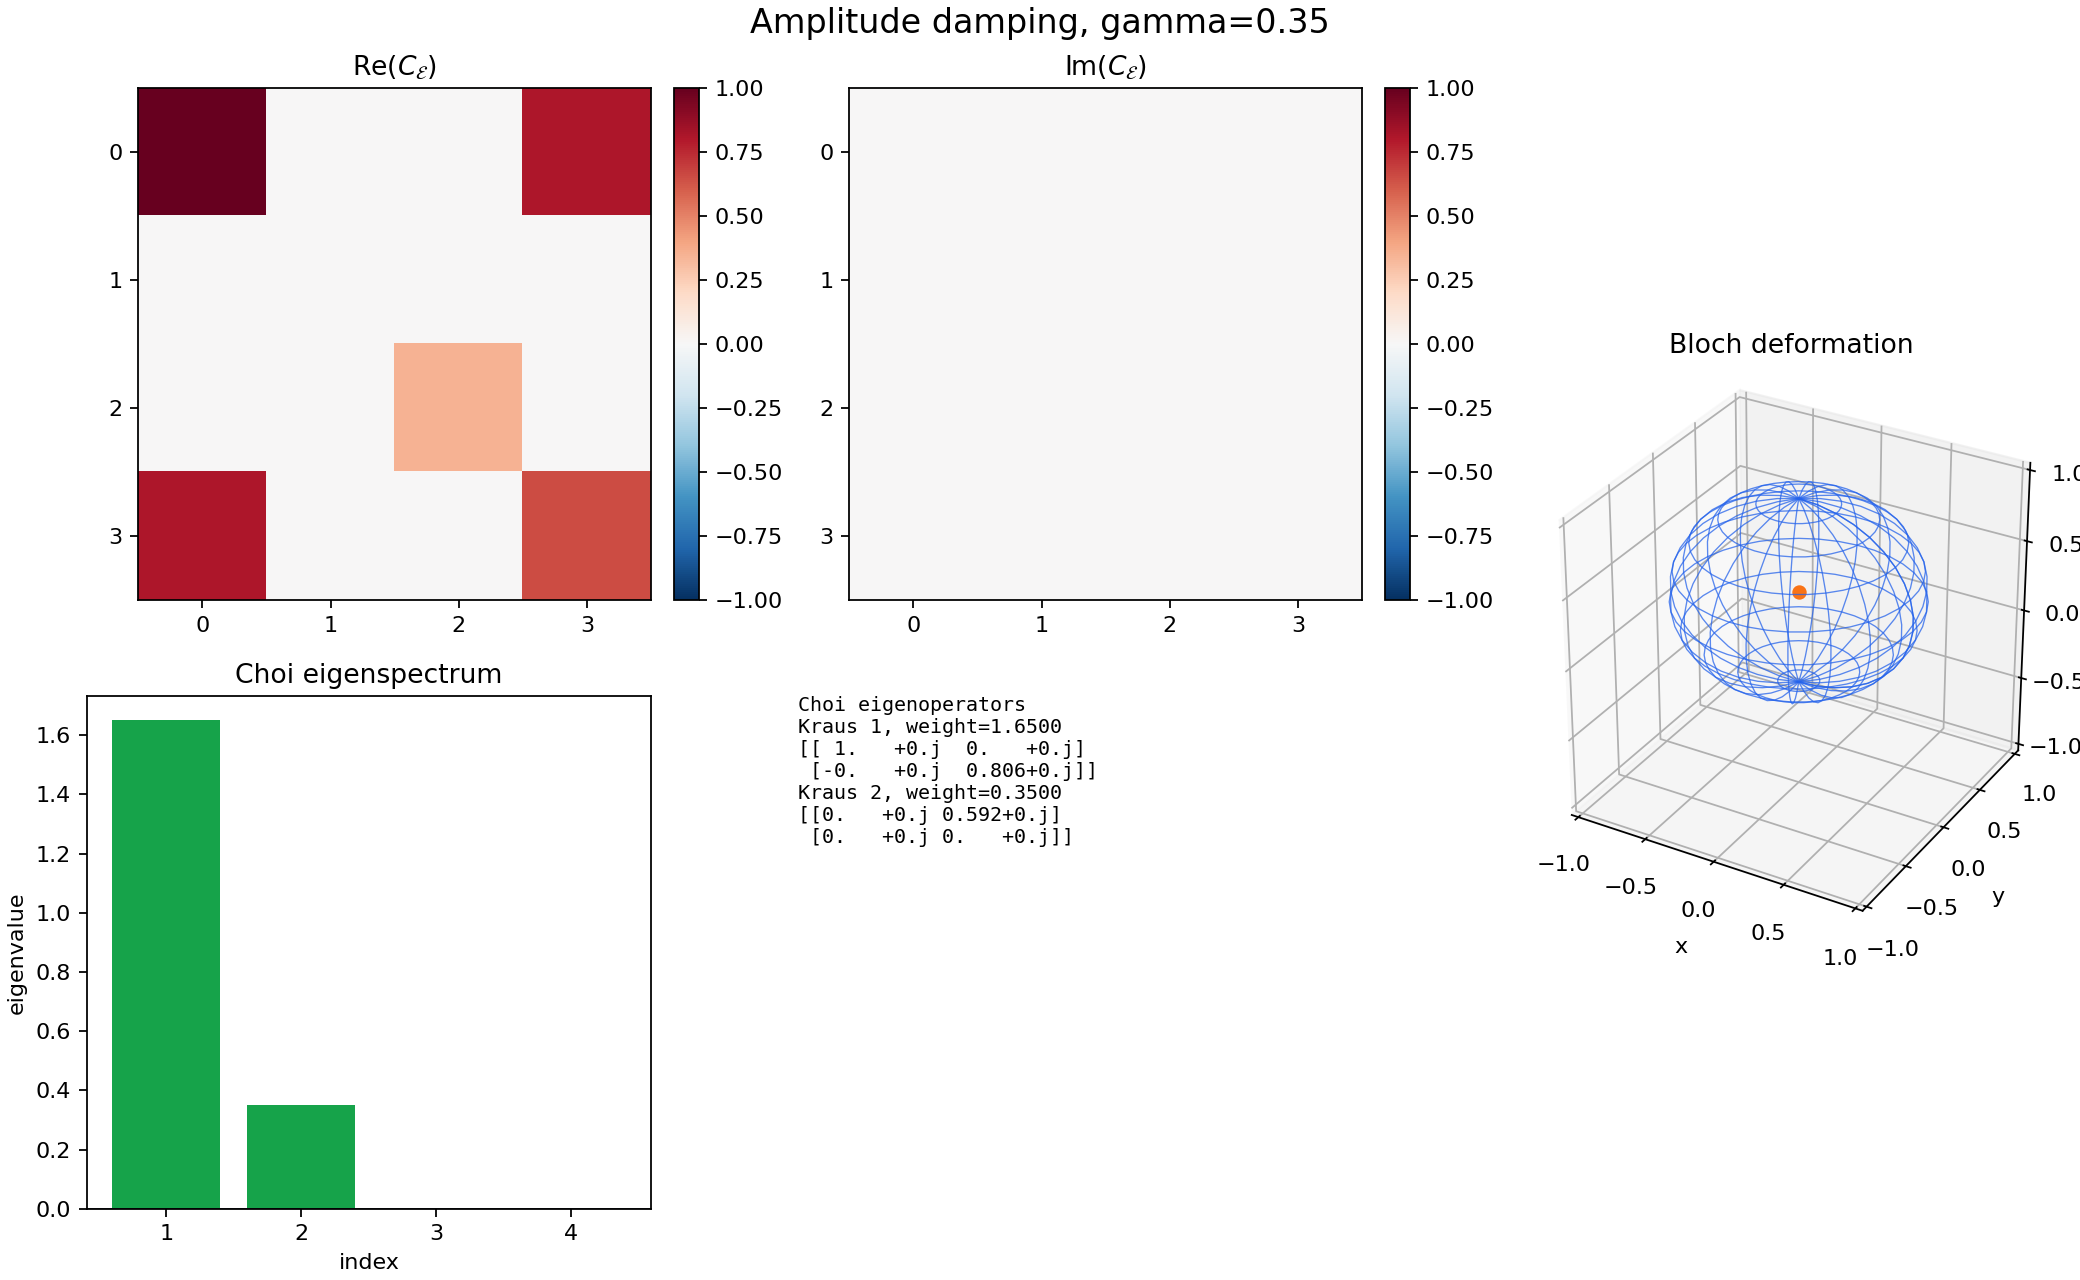
\includegraphics[width=0.94\textwidth]{fig_widget_dashboard.png}
\caption{Interactive widget의 amplitude damping 예시. 왼쪽에서는 Choi 행렬의 실수부, 허수부, 절댓값을 확인할 수 있고, 오른쪽에서는 Choi 고유값과 Bloch sphere 변형을 동시에 볼 수 있다. Amplitude damping에서는 Bloch sphere가 단순히 작아지는 것이 아니라 특정 방향으로 이동하므로, unital하지 않은 채널의 특징이 시각적으로 드러난다.}
\label{fig:widget-dashboard}
\end{figure}

그림 \ref{fig:widget-dashboard}에서 amplitude damping channel의 Bloch 구는 중심을 유지한 채 균일하게 작아지는 형태가 아니다. 이것이 depolarizing channel과 다른 점이다. depolarizing은 모든 방향의 Bloch 벡터를 비슷하게 줄이므로 완전 무질서 상태가 중심에 남지만, amplitude damping은 들뜬 상태가 바닥 상태로 내려가는 물리 과정이라 구의 중심 자체가 이동한다(2.5절의 unital 개념을 시각적으로 확인하는 셈이다).

Widget에서 CP 표시기가 Choi 고유값과 연결되어 있고, TP 표시기가 부분 대각합과 연결되어 있다는 점도 중요하다. 사용자가 매개변수를 바꿔 CP 영역 \emph{밖}으로 나가면 Choi 고유값 스펙트럼에 음의 고유값이 나타난다. 이때 행렬이 겉보기에는 작은 변화만 겪은 듯해도 물리적으로 가능한 채널은 아니게 된다(4.3절의 perturbed identity와 같은 현상). 따라서 widget은 단순한 시각화 도구라기보다, \emph{이론 조건(작업 1), tomography 진단(작업 2), 채널 차이 해석(작업 3)을 한 화면에서 묶는 장치}다. 이 점에서 widget 절은 별도의 부록이 아니라 프로젝트 전체를 다시 묶어 주는 마지막 연결 고리로 읽힌다.

%==================================================================
\section{통합 해석과 한계}
%==================================================================

\subsection{Choi 행렬은 어떻게 다섯 작업을 하나로 묶었나}

본 프로젝트의 가장 중요한 통합점은 Choi 행렬이 \emph{공통 인터페이스}로 작동했다는 것이다. 작업 1에서는 Choi 행렬이 채널 표현 변환과 CP/TP 판정의 기준이 되었다. 작업 2에서는 실험(또는 모의) tomography 데이터가 Choi 행렬로 재구성되며 fidelity와 잡음 진단의 출발점이 되었다. 작업 3에서는 두 Choi 행렬의 \emph{차이}가 SDP의 입력이 되어 최적 구별 확률로 이어졌다. 작업 4에서는 Choi 관점이 여러 time slot으로 확장되어 quantum comb가 되었고, 작업 5에서는 같은 조건들이 시각적 widget으로 표현되었다.

\begin{longtable}{p{0.18\textwidth}p{0.32\textwidth}p{0.38\textwidth}}
\toprule
파트 & Choi 행렬의 역할 & 결과 해석 \\
\midrule
이론 & 표현 변환과 CP/TP 판정 & 채널 formalism의 계산 기준을 세웠다. \\
Tomography & 재구성된 process의 표현 & fidelity와 noise diagnosis를 가능하게 했다. \\
SDP & channel difference의 최적화 입력 & diamond norm으로 구별 가능성을 계산했다. \\
Combs & generalized Choi operator & time correlation과 memory residue를 나타냈다. \\
Widget & 시각적 대시보드 & 고유값, partial trace, Bloch deformation을 연결했다. \\
\bottomrule
\caption{Choi 표현의 통합적 역할}
\label{tab:integration}
\end{longtable}

결과를 종합하면, Choi 행렬은 단순한 수학적 변환이 아니라 실험과 계산을 이어주는 \emph{좌표계}로 작동한다. 이론적으로는 물리성 조건(CP/TP)을 판정하고, 실험적으로는 재구성된 과정의 품질을 비교하며, 최적화에서는 실험적 성공확률을 계산하고, 시간 과정에서는 기억 구조를 드러낸다. 같은 행렬 표현을 끝까지 유지한 덕분에 각 주제의 결과가 서로 분리되지 않고 연결될 수 있었다.

\subsection{무엇을 조심해야 하는가}

한계도 분명하다. 첫째, 대부분의 예제는 1큐비트 또는 작은 2큐비트 계에 맞추어져 있다. Choi 행렬의 크기는 입력 차원과 출력 차원의 곱에 따라 커지고(예: 2큐비트면 $16\times16$), SDP 변수는 그 행렬 전체를 다루므로 큰 계에서는 계산 비용이 빠르게 증가한다. quantum comb도 time step 수가 늘면 차원이 \emph{지수적}으로 증가한다. 따라서 이 방법들은 개념적으로 강력하지만, 대규모 장치에 그대로 적용하려면 대칭성(symmetry), tensor network, 무작위화(randomized) 프로토콜 같은 추가 압축 기법이 필요하다.

둘째, process tomography 결과는 \emph{오프라인 모의 데이터}를 기반으로 한다(작업 2). 따라서 표에 제시된 fidelity와 diamond distance를 실제 IBM 하드웨어 성능으로 해석해서는 안 된다. 실제 하드웨어를 주장하려면 backend 이름, 보정 시각, shot 수, job ID, raw count 데이터, 불확실성 추정이 함께 제시되어야 한다. 본 보고서의 tomography 결과는 \emph{분석 파이프라인과 해석 방식의 검증}으로 보는 것이 적절하다.

%==================================================================
\section{결론}
%==================================================================

본 프로젝트는 Choi 표현이 왜 양자 채널 분석에서 강력한 도구인지를 여러 관점에서 확인했다.

\begin{itemize}
  \item \textbf{이론(작업 1):} Kraus, Choi, Stinespring, natural 표현이 machine precision 수준($10^{-16}$)에서 일관되게 변환됨을 보였다.
  \item \textbf{Tomography(작업 2):} 재구성된 Choi 행렬이 fidelity, diamond distance, Bloch 구 변형을 통해 잡음의 \emph{크기와 방향성}을 함께 드러냄을 확인했다.
  \item \textbf{SDP(작업 3):} diamond norm이 채널 구별 성공확률과 직접 연결되며, 얽힌 참조계와 반복 사용이 실제로 성능을 높일 수 있음을($0.75\to0.875\to0.969$) 보였다.
  \item \textbf{Quantum comb(작업 4):} 부분 채널이 멀쩡해 보여도 전체 다중 시점 과정에는 기억 상관이 남을 수 있음을 BLP/RHP 두 진단으로 확인했다.
  \item \textbf{Widget(작업 5):} 이 조건들을 한 화면에서 확인할 수 있게 하여 수식과 직관 사이의 간격을 줄였다.
\end{itemize}

전체적으로 Choi 행렬은 채널의 물리성, 실험적 재구성, 최적 구별, 시간 상관, 시각화를 \emph{하나의 언어}로 묶어 준다. 특히 CP 조건이 ``고유값이 음이 아님''으로, TP 조건이 ``부분 대각합이 항등행렬임''으로 바뀐다는 점은 계산과 해석 모두에서 큰 장점이다. 다만 계가 커질수록 Choi 행렬과 SDP의 크기가 빠르게 증가하므로, 앞으로는 더 효율적인 표현과 근사 방법을 함께 고려해야 한다.

\section*{참고문헌}
\addcontentsline{toc}{section}{참고문헌}

\begin{itemize}
  \item M. A. Nielsen and I. L. Chuang, \textit{Quantum Computation and Quantum Information}. Cambridge University Press, 2010.
  \item M.-D. Choi, ``Completely positive linear maps on complex matrices,'' \textit{Linear Algebra and its Applications}, 1975.
  \item A. Jamio{\l}kowski, ``Linear transformations which preserve trace and positive semidefiniteness of operators,'' \textit{Reports on Mathematical Physics}, 1972.
  \item J. Watrous, \textit{The Theory of Quantum Information}. Cambridge University Press, 2018.
  \item G. Chiribella, G. M. D'Ariano, and P. Perinotti, ``Quantum circuit architecture,'' \textit{Physical Review Letters}, 2008.
  \item H.-P. Breuer, E.-M. Laine, and J. Piilo, ``Measure for the degree of non-Markovian behavior of quantum processes,'' \textit{Physical Review Letters}, 2009.
\end{itemize}

\end{document}
